\section{Experimental Results}
\bigbreak
\subsection{Validation Test}
In order to check the validity of our implementation, we tested the output of our sequential and parallel programs with the output from MATLAB. The input was a $5000 \times 5000$ sparse matrix. The results are depicted in Figure \ref{fig:validation}. As we can see, the bandwidth has been significantly reduced in both sequential and parallel outputs. Also, bandwidth values are very close to the MATLAB bandwidth value. 
\begin{figure}[H]
    \centering
    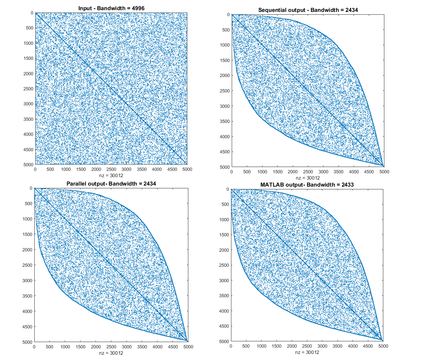
\includegraphics{Webp.net-resizeimage (2).jpg}
    \caption{Validation Benchmark}
    \label{fig:validation}
\end{figure}

\subsection{Execution Time Test}
Execution time benchmarking was performed on a DELL laptop with an Intel® Core™ i7-6500U CPU @ 2.50GHz × 4 processor and 8Gbytes RAM. Also, to test the scalability of our implementation we tested our parallel version on a more powerfull CPU AMD Ryzen7 4700 @ 2.0GHz x 8. Results are depicted in Figure \ref{fig:plot}. The inputs were sparse matrices with variable size and 1\% density. We observed that as density was increasing the speedup among the sequential and parallel implementation was also increasing. This is a reasonable observation, as a more dense matrix means that a node has more neighbours and as a result there are more iterations in the for loops that can be parallelized.
\begin{figure}[H]
    \centering
    %% Creator: Matplotlib, PGF backend
%%
%% To include the figure in your LaTeX document, write
%%   \input{<filename>.pgf}
%%
%% Make sure the required packages are loaded in your preamble
%%   \usepackage{pgf}
%%
%% Figures using additional raster images can only be included by \input if
%% they are in the same directory as the main LaTeX file. For loading figures
%% from other directories you can use the `import` package
%%   \usepackage{import}
%% and then include the figures with
%%   \import{<path to file>}{<filename>.pgf}
%%
%% Matplotlib used the following preamble
%%   \usepackage{fontspec}
%%   \setmainfont{DejaVuSerif.ttf}[Path=/home/evangelos/anaconda3/lib/python3.7/site-packages/matplotlib/mpl-data/fonts/ttf/]
%%   \setsansfont{DejaVuSans.ttf}[Path=/home/evangelos/anaconda3/lib/python3.7/site-packages/matplotlib/mpl-data/fonts/ttf/]
%%   \setmonofont{DejaVuSansMono.ttf}[Path=/home/evangelos/anaconda3/lib/python3.7/site-packages/matplotlib/mpl-data/fonts/ttf/]
%%
\begingroup%
\makeatletter%
\begin{pgfpicture}%
\pgfpathrectangle{\pgfpointorigin}{\pgfqpoint{6.590000in}{3.330000in}}%
\pgfusepath{use as bounding box, clip}%
\begin{pgfscope}%
\pgfsetbuttcap%
\pgfsetmiterjoin%
\definecolor{currentfill}{rgb}{1.000000,1.000000,1.000000}%
\pgfsetfillcolor{currentfill}%
\pgfsetlinewidth{0.000000pt}%
\definecolor{currentstroke}{rgb}{1.000000,1.000000,1.000000}%
\pgfsetstrokecolor{currentstroke}%
\pgfsetdash{}{0pt}%
\pgfpathmoveto{\pgfqpoint{0.000000in}{0.000000in}}%
\pgfpathlineto{\pgfqpoint{6.590000in}{0.000000in}}%
\pgfpathlineto{\pgfqpoint{6.590000in}{3.330000in}}%
\pgfpathlineto{\pgfqpoint{0.000000in}{3.330000in}}%
\pgfpathclose%
\pgfusepath{fill}%
\end{pgfscope}%
\begin{pgfscope}%
\pgfsetbuttcap%
\pgfsetmiterjoin%
\definecolor{currentfill}{rgb}{1.000000,1.000000,1.000000}%
\pgfsetfillcolor{currentfill}%
\pgfsetlinewidth{0.000000pt}%
\definecolor{currentstroke}{rgb}{0.000000,0.000000,0.000000}%
\pgfsetstrokecolor{currentstroke}%
\pgfsetstrokeopacity{0.000000}%
\pgfsetdash{}{0pt}%
\pgfpathmoveto{\pgfqpoint{0.664028in}{0.582778in}}%
\pgfpathlineto{\pgfqpoint{6.405000in}{0.582778in}}%
\pgfpathlineto{\pgfqpoint{6.405000in}{2.976667in}}%
\pgfpathlineto{\pgfqpoint{0.664028in}{2.976667in}}%
\pgfpathclose%
\pgfusepath{fill}%
\end{pgfscope}%
\begin{pgfscope}%
\pgfpathrectangle{\pgfqpoint{0.664028in}{0.582778in}}{\pgfqpoint{5.740972in}{2.393889in}}%
\pgfusepath{clip}%
\pgfsetroundcap%
\pgfsetroundjoin%
\pgfsetlinewidth{0.803000pt}%
\definecolor{currentstroke}{rgb}{0.800000,0.800000,0.800000}%
\pgfsetstrokecolor{currentstroke}%
\pgfsetdash{}{0pt}%
\pgfpathmoveto{\pgfqpoint{1.399442in}{0.582778in}}%
\pgfpathlineto{\pgfqpoint{1.399442in}{2.976667in}}%
\pgfusepath{stroke}%
\end{pgfscope}%
\begin{pgfscope}%
\definecolor{textcolor}{rgb}{0.150000,0.150000,0.150000}%
\pgfsetstrokecolor{textcolor}%
\pgfsetfillcolor{textcolor}%
\pgftext[x=1.399442in,y=0.485556in,,top]{\color{textcolor}\sffamily\fontsize{10.000000}{12.000000}\selectfont 5000}%
\end{pgfscope}%
\begin{pgfscope}%
\pgfpathrectangle{\pgfqpoint{0.664028in}{0.582778in}}{\pgfqpoint{5.740972in}{2.393889in}}%
\pgfusepath{clip}%
\pgfsetroundcap%
\pgfsetroundjoin%
\pgfsetlinewidth{0.803000pt}%
\definecolor{currentstroke}{rgb}{0.800000,0.800000,0.800000}%
\pgfsetstrokecolor{currentstroke}%
\pgfsetdash{}{0pt}%
\pgfpathmoveto{\pgfqpoint{2.348363in}{0.582778in}}%
\pgfpathlineto{\pgfqpoint{2.348363in}{2.976667in}}%
\pgfusepath{stroke}%
\end{pgfscope}%
\begin{pgfscope}%
\definecolor{textcolor}{rgb}{0.150000,0.150000,0.150000}%
\pgfsetstrokecolor{textcolor}%
\pgfsetfillcolor{textcolor}%
\pgftext[x=2.348363in,y=0.485556in,,top]{\color{textcolor}\sffamily\fontsize{10.000000}{12.000000}\selectfont 10000}%
\end{pgfscope}%
\begin{pgfscope}%
\pgfpathrectangle{\pgfqpoint{0.664028in}{0.582778in}}{\pgfqpoint{5.740972in}{2.393889in}}%
\pgfusepath{clip}%
\pgfsetroundcap%
\pgfsetroundjoin%
\pgfsetlinewidth{0.803000pt}%
\definecolor{currentstroke}{rgb}{0.800000,0.800000,0.800000}%
\pgfsetstrokecolor{currentstroke}%
\pgfsetdash{}{0pt}%
\pgfpathmoveto{\pgfqpoint{3.297284in}{0.582778in}}%
\pgfpathlineto{\pgfqpoint{3.297284in}{2.976667in}}%
\pgfusepath{stroke}%
\end{pgfscope}%
\begin{pgfscope}%
\definecolor{textcolor}{rgb}{0.150000,0.150000,0.150000}%
\pgfsetstrokecolor{textcolor}%
\pgfsetfillcolor{textcolor}%
\pgftext[x=3.297284in,y=0.485556in,,top]{\color{textcolor}\sffamily\fontsize{10.000000}{12.000000}\selectfont 15000}%
\end{pgfscope}%
\begin{pgfscope}%
\pgfpathrectangle{\pgfqpoint{0.664028in}{0.582778in}}{\pgfqpoint{5.740972in}{2.393889in}}%
\pgfusepath{clip}%
\pgfsetroundcap%
\pgfsetroundjoin%
\pgfsetlinewidth{0.803000pt}%
\definecolor{currentstroke}{rgb}{0.800000,0.800000,0.800000}%
\pgfsetstrokecolor{currentstroke}%
\pgfsetdash{}{0pt}%
\pgfpathmoveto{\pgfqpoint{4.246205in}{0.582778in}}%
\pgfpathlineto{\pgfqpoint{4.246205in}{2.976667in}}%
\pgfusepath{stroke}%
\end{pgfscope}%
\begin{pgfscope}%
\definecolor{textcolor}{rgb}{0.150000,0.150000,0.150000}%
\pgfsetstrokecolor{textcolor}%
\pgfsetfillcolor{textcolor}%
\pgftext[x=4.246205in,y=0.485556in,,top]{\color{textcolor}\sffamily\fontsize{10.000000}{12.000000}\selectfont 20000}%
\end{pgfscope}%
\begin{pgfscope}%
\pgfpathrectangle{\pgfqpoint{0.664028in}{0.582778in}}{\pgfqpoint{5.740972in}{2.393889in}}%
\pgfusepath{clip}%
\pgfsetroundcap%
\pgfsetroundjoin%
\pgfsetlinewidth{0.803000pt}%
\definecolor{currentstroke}{rgb}{0.800000,0.800000,0.800000}%
\pgfsetstrokecolor{currentstroke}%
\pgfsetdash{}{0pt}%
\pgfpathmoveto{\pgfqpoint{5.195126in}{0.582778in}}%
\pgfpathlineto{\pgfqpoint{5.195126in}{2.976667in}}%
\pgfusepath{stroke}%
\end{pgfscope}%
\begin{pgfscope}%
\definecolor{textcolor}{rgb}{0.150000,0.150000,0.150000}%
\pgfsetstrokecolor{textcolor}%
\pgfsetfillcolor{textcolor}%
\pgftext[x=5.195126in,y=0.485556in,,top]{\color{textcolor}\sffamily\fontsize{10.000000}{12.000000}\selectfont 25000}%
\end{pgfscope}%
\begin{pgfscope}%
\pgfpathrectangle{\pgfqpoint{0.664028in}{0.582778in}}{\pgfqpoint{5.740972in}{2.393889in}}%
\pgfusepath{clip}%
\pgfsetroundcap%
\pgfsetroundjoin%
\pgfsetlinewidth{0.803000pt}%
\definecolor{currentstroke}{rgb}{0.800000,0.800000,0.800000}%
\pgfsetstrokecolor{currentstroke}%
\pgfsetdash{}{0pt}%
\pgfpathmoveto{\pgfqpoint{6.144047in}{0.582778in}}%
\pgfpathlineto{\pgfqpoint{6.144047in}{2.976667in}}%
\pgfusepath{stroke}%
\end{pgfscope}%
\begin{pgfscope}%
\definecolor{textcolor}{rgb}{0.150000,0.150000,0.150000}%
\pgfsetstrokecolor{textcolor}%
\pgfsetfillcolor{textcolor}%
\pgftext[x=6.144047in,y=0.485556in,,top]{\color{textcolor}\sffamily\fontsize{10.000000}{12.000000}\selectfont 30000}%
\end{pgfscope}%
\begin{pgfscope}%
\definecolor{textcolor}{rgb}{0.150000,0.150000,0.150000}%
\pgfsetstrokecolor{textcolor}%
\pgfsetfillcolor{textcolor}%
\pgftext[x=3.534514in,y=0.295587in,,top]{\color{textcolor}\sffamily\fontsize{10.000000}{12.000000}\selectfont Size - n}%
\end{pgfscope}%
\begin{pgfscope}%
\pgfpathrectangle{\pgfqpoint{0.664028in}{0.582778in}}{\pgfqpoint{5.740972in}{2.393889in}}%
\pgfusepath{clip}%
\pgfsetroundcap%
\pgfsetroundjoin%
\pgfsetlinewidth{0.803000pt}%
\definecolor{currentstroke}{rgb}{0.800000,0.800000,0.800000}%
\pgfsetstrokecolor{currentstroke}%
\pgfsetdash{}{0pt}%
\pgfpathmoveto{\pgfqpoint{0.664028in}{0.676500in}}%
\pgfpathlineto{\pgfqpoint{6.405000in}{0.676500in}}%
\pgfusepath{stroke}%
\end{pgfscope}%
\begin{pgfscope}%
\definecolor{textcolor}{rgb}{0.150000,0.150000,0.150000}%
\pgfsetstrokecolor{textcolor}%
\pgfsetfillcolor{textcolor}%
\pgftext[x=0.345926in,y=0.623738in,left,base]{\color{textcolor}\sffamily\fontsize{10.000000}{12.000000}\selectfont 0.0}%
\end{pgfscope}%
\begin{pgfscope}%
\pgfpathrectangle{\pgfqpoint{0.664028in}{0.582778in}}{\pgfqpoint{5.740972in}{2.393889in}}%
\pgfusepath{clip}%
\pgfsetroundcap%
\pgfsetroundjoin%
\pgfsetlinewidth{0.803000pt}%
\definecolor{currentstroke}{rgb}{0.800000,0.800000,0.800000}%
\pgfsetstrokecolor{currentstroke}%
\pgfsetdash{}{0pt}%
\pgfpathmoveto{\pgfqpoint{0.664028in}{0.983105in}}%
\pgfpathlineto{\pgfqpoint{6.405000in}{0.983105in}}%
\pgfusepath{stroke}%
\end{pgfscope}%
\begin{pgfscope}%
\definecolor{textcolor}{rgb}{0.150000,0.150000,0.150000}%
\pgfsetstrokecolor{textcolor}%
\pgfsetfillcolor{textcolor}%
\pgftext[x=0.345926in,y=0.930343in,left,base]{\color{textcolor}\sffamily\fontsize{10.000000}{12.000000}\selectfont 0.5}%
\end{pgfscope}%
\begin{pgfscope}%
\pgfpathrectangle{\pgfqpoint{0.664028in}{0.582778in}}{\pgfqpoint{5.740972in}{2.393889in}}%
\pgfusepath{clip}%
\pgfsetroundcap%
\pgfsetroundjoin%
\pgfsetlinewidth{0.803000pt}%
\definecolor{currentstroke}{rgb}{0.800000,0.800000,0.800000}%
\pgfsetstrokecolor{currentstroke}%
\pgfsetdash{}{0pt}%
\pgfpathmoveto{\pgfqpoint{0.664028in}{1.289709in}}%
\pgfpathlineto{\pgfqpoint{6.405000in}{1.289709in}}%
\pgfusepath{stroke}%
\end{pgfscope}%
\begin{pgfscope}%
\definecolor{textcolor}{rgb}{0.150000,0.150000,0.150000}%
\pgfsetstrokecolor{textcolor}%
\pgfsetfillcolor{textcolor}%
\pgftext[x=0.345926in,y=1.236948in,left,base]{\color{textcolor}\sffamily\fontsize{10.000000}{12.000000}\selectfont 1.0}%
\end{pgfscope}%
\begin{pgfscope}%
\pgfpathrectangle{\pgfqpoint{0.664028in}{0.582778in}}{\pgfqpoint{5.740972in}{2.393889in}}%
\pgfusepath{clip}%
\pgfsetroundcap%
\pgfsetroundjoin%
\pgfsetlinewidth{0.803000pt}%
\definecolor{currentstroke}{rgb}{0.800000,0.800000,0.800000}%
\pgfsetstrokecolor{currentstroke}%
\pgfsetdash{}{0pt}%
\pgfpathmoveto{\pgfqpoint{0.664028in}{1.596314in}}%
\pgfpathlineto{\pgfqpoint{6.405000in}{1.596314in}}%
\pgfusepath{stroke}%
\end{pgfscope}%
\begin{pgfscope}%
\definecolor{textcolor}{rgb}{0.150000,0.150000,0.150000}%
\pgfsetstrokecolor{textcolor}%
\pgfsetfillcolor{textcolor}%
\pgftext[x=0.345926in,y=1.543553in,left,base]{\color{textcolor}\sffamily\fontsize{10.000000}{12.000000}\selectfont 1.5}%
\end{pgfscope}%
\begin{pgfscope}%
\pgfpathrectangle{\pgfqpoint{0.664028in}{0.582778in}}{\pgfqpoint{5.740972in}{2.393889in}}%
\pgfusepath{clip}%
\pgfsetroundcap%
\pgfsetroundjoin%
\pgfsetlinewidth{0.803000pt}%
\definecolor{currentstroke}{rgb}{0.800000,0.800000,0.800000}%
\pgfsetstrokecolor{currentstroke}%
\pgfsetdash{}{0pt}%
\pgfpathmoveto{\pgfqpoint{0.664028in}{1.902919in}}%
\pgfpathlineto{\pgfqpoint{6.405000in}{1.902919in}}%
\pgfusepath{stroke}%
\end{pgfscope}%
\begin{pgfscope}%
\definecolor{textcolor}{rgb}{0.150000,0.150000,0.150000}%
\pgfsetstrokecolor{textcolor}%
\pgfsetfillcolor{textcolor}%
\pgftext[x=0.345926in,y=1.850158in,left,base]{\color{textcolor}\sffamily\fontsize{10.000000}{12.000000}\selectfont 2.0}%
\end{pgfscope}%
\begin{pgfscope}%
\pgfpathrectangle{\pgfqpoint{0.664028in}{0.582778in}}{\pgfqpoint{5.740972in}{2.393889in}}%
\pgfusepath{clip}%
\pgfsetroundcap%
\pgfsetroundjoin%
\pgfsetlinewidth{0.803000pt}%
\definecolor{currentstroke}{rgb}{0.800000,0.800000,0.800000}%
\pgfsetstrokecolor{currentstroke}%
\pgfsetdash{}{0pt}%
\pgfpathmoveto{\pgfqpoint{0.664028in}{2.209524in}}%
\pgfpathlineto{\pgfqpoint{6.405000in}{2.209524in}}%
\pgfusepath{stroke}%
\end{pgfscope}%
\begin{pgfscope}%
\definecolor{textcolor}{rgb}{0.150000,0.150000,0.150000}%
\pgfsetstrokecolor{textcolor}%
\pgfsetfillcolor{textcolor}%
\pgftext[x=0.345926in,y=2.156762in,left,base]{\color{textcolor}\sffamily\fontsize{10.000000}{12.000000}\selectfont 2.5}%
\end{pgfscope}%
\begin{pgfscope}%
\pgfpathrectangle{\pgfqpoint{0.664028in}{0.582778in}}{\pgfqpoint{5.740972in}{2.393889in}}%
\pgfusepath{clip}%
\pgfsetroundcap%
\pgfsetroundjoin%
\pgfsetlinewidth{0.803000pt}%
\definecolor{currentstroke}{rgb}{0.800000,0.800000,0.800000}%
\pgfsetstrokecolor{currentstroke}%
\pgfsetdash{}{0pt}%
\pgfpathmoveto{\pgfqpoint{0.664028in}{2.516129in}}%
\pgfpathlineto{\pgfqpoint{6.405000in}{2.516129in}}%
\pgfusepath{stroke}%
\end{pgfscope}%
\begin{pgfscope}%
\definecolor{textcolor}{rgb}{0.150000,0.150000,0.150000}%
\pgfsetstrokecolor{textcolor}%
\pgfsetfillcolor{textcolor}%
\pgftext[x=0.345926in,y=2.463367in,left,base]{\color{textcolor}\sffamily\fontsize{10.000000}{12.000000}\selectfont 3.0}%
\end{pgfscope}%
\begin{pgfscope}%
\pgfpathrectangle{\pgfqpoint{0.664028in}{0.582778in}}{\pgfqpoint{5.740972in}{2.393889in}}%
\pgfusepath{clip}%
\pgfsetroundcap%
\pgfsetroundjoin%
\pgfsetlinewidth{0.803000pt}%
\definecolor{currentstroke}{rgb}{0.800000,0.800000,0.800000}%
\pgfsetstrokecolor{currentstroke}%
\pgfsetdash{}{0pt}%
\pgfpathmoveto{\pgfqpoint{0.664028in}{2.822734in}}%
\pgfpathlineto{\pgfqpoint{6.405000in}{2.822734in}}%
\pgfusepath{stroke}%
\end{pgfscope}%
\begin{pgfscope}%
\definecolor{textcolor}{rgb}{0.150000,0.150000,0.150000}%
\pgfsetstrokecolor{textcolor}%
\pgfsetfillcolor{textcolor}%
\pgftext[x=0.345926in,y=2.769972in,left,base]{\color{textcolor}\sffamily\fontsize{10.000000}{12.000000}\selectfont 3.5}%
\end{pgfscope}%
\begin{pgfscope}%
\definecolor{textcolor}{rgb}{0.150000,0.150000,0.150000}%
\pgfsetstrokecolor{textcolor}%
\pgfsetfillcolor{textcolor}%
\pgftext[x=0.290371in,y=1.779722in,,bottom,rotate=90.000000]{\color{textcolor}\sffamily\fontsize{10.000000}{12.000000}\selectfont Execution Time (seconds)}%
\end{pgfscope}%
\begin{pgfscope}%
\pgfpathrectangle{\pgfqpoint{0.664028in}{0.582778in}}{\pgfqpoint{5.740972in}{2.393889in}}%
\pgfusepath{clip}%
\pgfsetroundcap%
\pgfsetroundjoin%
\pgfsetlinewidth{1.505625pt}%
\definecolor{currentstroke}{rgb}{0.000000,0.501961,0.000000}%
\pgfsetstrokecolor{currentstroke}%
\pgfsetdash{}{0pt}%
\pgfpathmoveto{\pgfqpoint{0.924981in}{0.694570in}}%
\pgfpathlineto{\pgfqpoint{1.399442in}{0.745931in}}%
\pgfpathlineto{\pgfqpoint{1.873902in}{0.817959in}}%
\pgfpathlineto{\pgfqpoint{2.348363in}{0.939310in}}%
\pgfpathlineto{\pgfqpoint{2.822823in}{1.058938in}}%
\pgfpathlineto{\pgfqpoint{3.297284in}{1.225850in}}%
\pgfpathlineto{\pgfqpoint{3.771744in}{1.421004in}}%
\pgfpathlineto{\pgfqpoint{4.246205in}{1.649620in}}%
\pgfpathlineto{\pgfqpoint{4.720665in}{1.910220in}}%
\pgfpathlineto{\pgfqpoint{5.195126in}{2.197716in}}%
\pgfpathlineto{\pgfqpoint{6.144047in}{2.867854in}}%
\pgfusepath{stroke}%
\end{pgfscope}%
\begin{pgfscope}%
\pgfpathrectangle{\pgfqpoint{0.664028in}{0.582778in}}{\pgfqpoint{5.740972in}{2.393889in}}%
\pgfusepath{clip}%
\pgfsetroundcap%
\pgfsetroundjoin%
\pgfsetlinewidth{1.505625pt}%
\definecolor{currentstroke}{rgb}{1.000000,0.000000,0.000000}%
\pgfsetstrokecolor{currentstroke}%
\pgfsetdash{}{0pt}%
\pgfpathmoveto{\pgfqpoint{0.924981in}{0.691591in}}%
\pgfpathlineto{\pgfqpoint{1.399442in}{0.721571in}}%
\pgfpathlineto{\pgfqpoint{1.873902in}{0.763581in}}%
\pgfpathlineto{\pgfqpoint{2.348363in}{0.839960in}}%
\pgfpathlineto{\pgfqpoint{2.822823in}{0.915457in}}%
\pgfpathlineto{\pgfqpoint{3.297284in}{0.997879in}}%
\pgfpathlineto{\pgfqpoint{3.771744in}{1.122401in}}%
\pgfpathlineto{\pgfqpoint{4.246205in}{1.250172in}}%
\pgfpathlineto{\pgfqpoint{4.720665in}{1.412953in}}%
\pgfpathlineto{\pgfqpoint{5.195126in}{1.566571in}}%
\pgfpathlineto{\pgfqpoint{6.144047in}{1.987378in}}%
\pgfusepath{stroke}%
\end{pgfscope}%
\begin{pgfscope}%
\pgfpathrectangle{\pgfqpoint{0.664028in}{0.582778in}}{\pgfqpoint{5.740972in}{2.393889in}}%
\pgfusepath{clip}%
\pgfsetroundcap%
\pgfsetroundjoin%
\pgfsetlinewidth{1.505625pt}%
\definecolor{currentstroke}{rgb}{0.254902,0.411765,0.882353}%
\pgfsetstrokecolor{currentstroke}%
\pgfsetdash{}{0pt}%
\pgfpathmoveto{\pgfqpoint{1.399442in}{0.712679in}}%
\pgfpathlineto{\pgfqpoint{2.348363in}{0.841407in}}%
\pgfpathlineto{\pgfqpoint{3.297284in}{1.036897in}}%
\pgfpathlineto{\pgfqpoint{4.246205in}{1.368807in}}%
\pgfpathlineto{\pgfqpoint{5.195126in}{1.650107in}}%
\pgfpathlineto{\pgfqpoint{6.144047in}{2.104659in}}%
\pgfusepath{stroke}%
\end{pgfscope}%
\begin{pgfscope}%
\pgfpathrectangle{\pgfqpoint{0.664028in}{0.582778in}}{\pgfqpoint{5.740972in}{2.393889in}}%
\pgfusepath{clip}%
\pgfsetroundcap%
\pgfsetroundjoin%
\pgfsetlinewidth{1.505625pt}%
\definecolor{currentstroke}{rgb}{1.000000,0.647059,0.000000}%
\pgfsetstrokecolor{currentstroke}%
\pgfsetdash{}{0pt}%
\pgfpathmoveto{\pgfqpoint{1.399442in}{0.710226in}}%
\pgfpathlineto{\pgfqpoint{2.348363in}{0.778293in}}%
\pgfpathlineto{\pgfqpoint{3.297284in}{0.875180in}}%
\pgfpathlineto{\pgfqpoint{4.246205in}{1.044426in}}%
\pgfpathlineto{\pgfqpoint{5.195126in}{1.068954in}}%
\pgfpathlineto{\pgfqpoint{6.144047in}{1.203860in}}%
\pgfusepath{stroke}%
\end{pgfscope}%
\begin{pgfscope}%
\pgfsetrectcap%
\pgfsetmiterjoin%
\pgfsetlinewidth{0.803000pt}%
\definecolor{currentstroke}{rgb}{0.800000,0.800000,0.800000}%
\pgfsetstrokecolor{currentstroke}%
\pgfsetdash{}{0pt}%
\pgfpathmoveto{\pgfqpoint{0.664028in}{0.582778in}}%
\pgfpathlineto{\pgfqpoint{0.664028in}{2.976667in}}%
\pgfusepath{stroke}%
\end{pgfscope}%
\begin{pgfscope}%
\pgfsetrectcap%
\pgfsetmiterjoin%
\pgfsetlinewidth{0.803000pt}%
\definecolor{currentstroke}{rgb}{0.800000,0.800000,0.800000}%
\pgfsetstrokecolor{currentstroke}%
\pgfsetdash{}{0pt}%
\pgfpathmoveto{\pgfqpoint{6.405000in}{0.582778in}}%
\pgfpathlineto{\pgfqpoint{6.405000in}{2.976667in}}%
\pgfusepath{stroke}%
\end{pgfscope}%
\begin{pgfscope}%
\pgfsetrectcap%
\pgfsetmiterjoin%
\pgfsetlinewidth{0.803000pt}%
\definecolor{currentstroke}{rgb}{0.800000,0.800000,0.800000}%
\pgfsetstrokecolor{currentstroke}%
\pgfsetdash{}{0pt}%
\pgfpathmoveto{\pgfqpoint{0.664028in}{0.582778in}}%
\pgfpathlineto{\pgfqpoint{6.405000in}{0.582778in}}%
\pgfusepath{stroke}%
\end{pgfscope}%
\begin{pgfscope}%
\pgfsetrectcap%
\pgfsetmiterjoin%
\pgfsetlinewidth{0.803000pt}%
\definecolor{currentstroke}{rgb}{0.800000,0.800000,0.800000}%
\pgfsetstrokecolor{currentstroke}%
\pgfsetdash{}{0pt}%
\pgfpathmoveto{\pgfqpoint{0.664028in}{2.976667in}}%
\pgfpathlineto{\pgfqpoint{6.405000in}{2.976667in}}%
\pgfusepath{stroke}%
\end{pgfscope}%
\begin{pgfscope}%
\definecolor{textcolor}{rgb}{0.150000,0.150000,0.150000}%
\pgfsetstrokecolor{textcolor}%
\pgfsetfillcolor{textcolor}%
\pgftext[x=3.534514in,y=3.060000in,,base]{\color{textcolor}\sffamily\fontsize{12.000000}{14.400000}\selectfont Execution Time Benchmark}%
\end{pgfscope}%
\begin{pgfscope}%
\pgfsetbuttcap%
\pgfsetmiterjoin%
\definecolor{currentfill}{rgb}{1.000000,1.000000,1.000000}%
\pgfsetfillcolor{currentfill}%
\pgfsetfillopacity{0.800000}%
\pgfsetlinewidth{1.003750pt}%
\definecolor{currentstroke}{rgb}{0.800000,0.800000,0.800000}%
\pgfsetstrokecolor{currentstroke}%
\pgfsetstrokeopacity{0.800000}%
\pgfsetdash{}{0pt}%
\pgfpathmoveto{\pgfqpoint{0.761250in}{1.846269in}}%
\pgfpathlineto{\pgfqpoint{3.996968in}{1.846269in}}%
\pgfpathquadraticcurveto{\pgfqpoint{4.024746in}{1.846269in}}{\pgfqpoint{4.024746in}{1.874047in}}%
\pgfpathlineto{\pgfqpoint{4.024746in}{2.879444in}}%
\pgfpathquadraticcurveto{\pgfqpoint{4.024746in}{2.907222in}}{\pgfqpoint{3.996968in}{2.907222in}}%
\pgfpathlineto{\pgfqpoint{0.761250in}{2.907222in}}%
\pgfpathquadraticcurveto{\pgfqpoint{0.733472in}{2.907222in}}{\pgfqpoint{0.733472in}{2.879444in}}%
\pgfpathlineto{\pgfqpoint{0.733472in}{1.874047in}}%
\pgfpathquadraticcurveto{\pgfqpoint{0.733472in}{1.846269in}}{\pgfqpoint{0.761250in}{1.846269in}}%
\pgfpathclose%
\pgfusepath{stroke,fill}%
\end{pgfscope}%
\begin{pgfscope}%
\pgfsetroundcap%
\pgfsetroundjoin%
\pgfsetlinewidth{0.000000pt}%
\definecolor{currentstroke}{rgb}{1.000000,1.000000,1.000000}%
\pgfsetstrokecolor{currentstroke}%
\pgfsetdash{}{0pt}%
\pgfpathmoveto{\pgfqpoint{0.789028in}{2.794755in}}%
\pgfpathlineto{\pgfqpoint{1.066806in}{2.794755in}}%
\pgfusepath{}%
\end{pgfscope}%
\begin{pgfscope}%
\definecolor{textcolor}{rgb}{0.150000,0.150000,0.150000}%
\pgfsetstrokecolor{textcolor}%
\pgfsetfillcolor{textcolor}%
\pgftext[x=1.177917in,y=2.746144in,left,base]{\color{textcolor}\sffamily\fontsize{10.000000}{12.000000}\selectfont type}%
\end{pgfscope}%
\begin{pgfscope}%
\pgfsetroundcap%
\pgfsetroundjoin%
\pgfsetlinewidth{1.505625pt}%
\definecolor{currentstroke}{rgb}{0.000000,0.501961,0.000000}%
\pgfsetstrokecolor{currentstroke}%
\pgfsetdash{}{0pt}%
\pgfpathmoveto{\pgfqpoint{0.789028in}{2.590897in}}%
\pgfpathlineto{\pgfqpoint{1.066806in}{2.590897in}}%
\pgfusepath{stroke}%
\end{pgfscope}%
\begin{pgfscope}%
\definecolor{textcolor}{rgb}{0.150000,0.150000,0.150000}%
\pgfsetstrokecolor{textcolor}%
\pgfsetfillcolor{textcolor}%
\pgftext[x=1.177917in,y=2.542286in,left,base]{\color{textcolor}\sffamily\fontsize{10.000000}{12.000000}\selectfont sequential intel i7 @ 2.5GHz x 4}%
\end{pgfscope}%
\begin{pgfscope}%
\pgfsetroundcap%
\pgfsetroundjoin%
\pgfsetlinewidth{1.505625pt}%
\definecolor{currentstroke}{rgb}{1.000000,0.000000,0.000000}%
\pgfsetstrokecolor{currentstroke}%
\pgfsetdash{}{0pt}%
\pgfpathmoveto{\pgfqpoint{0.789028in}{2.387040in}}%
\pgfpathlineto{\pgfqpoint{1.066806in}{2.387040in}}%
\pgfusepath{stroke}%
\end{pgfscope}%
\begin{pgfscope}%
\definecolor{textcolor}{rgb}{0.150000,0.150000,0.150000}%
\pgfsetstrokecolor{textcolor}%
\pgfsetfillcolor{textcolor}%
\pgftext[x=1.177917in,y=2.338429in,left,base]{\color{textcolor}\sffamily\fontsize{10.000000}{12.000000}\selectfont parallel intel i7 @ 2.5GHz x 4}%
\end{pgfscope}%
\begin{pgfscope}%
\pgfsetroundcap%
\pgfsetroundjoin%
\pgfsetlinewidth{1.505625pt}%
\definecolor{currentstroke}{rgb}{0.254902,0.411765,0.882353}%
\pgfsetstrokecolor{currentstroke}%
\pgfsetdash{}{0pt}%
\pgfpathmoveto{\pgfqpoint{0.789028in}{2.183183in}}%
\pgfpathlineto{\pgfqpoint{1.066806in}{2.183183in}}%
\pgfusepath{stroke}%
\end{pgfscope}%
\begin{pgfscope}%
\definecolor{textcolor}{rgb}{0.150000,0.150000,0.150000}%
\pgfsetstrokecolor{textcolor}%
\pgfsetfillcolor{textcolor}%
\pgftext[x=1.177917in,y=2.134572in,left,base]{\color{textcolor}\sffamily\fontsize{10.000000}{12.000000}\selectfont MATLAB intel i7 @ 2.5GHz x 4}%
\end{pgfscope}%
\begin{pgfscope}%
\pgfsetroundcap%
\pgfsetroundjoin%
\pgfsetlinewidth{1.505625pt}%
\definecolor{currentstroke}{rgb}{1.000000,0.647059,0.000000}%
\pgfsetstrokecolor{currentstroke}%
\pgfsetdash{}{0pt}%
\pgfpathmoveto{\pgfqpoint{0.789028in}{1.979326in}}%
\pgfpathlineto{\pgfqpoint{1.066806in}{1.979326in}}%
\pgfusepath{stroke}%
\end{pgfscope}%
\begin{pgfscope}%
\definecolor{textcolor}{rgb}{0.150000,0.150000,0.150000}%
\pgfsetstrokecolor{textcolor}%
\pgfsetfillcolor{textcolor}%
\pgftext[x=1.177917in,y=1.930715in,left,base]{\color{textcolor}\sffamily\fontsize{10.000000}{12.000000}\selectfont parallel AMD Ryzen7 4700U @ 2GHz x 8}%
\end{pgfscope}%
\end{pgfpicture}%
\makeatother%
\endgroup%

    \caption{Execution Time Benchmark}
    \label{fig:plot}
\end{figure}
